\documentclass[11pt,a4paper]{article}
\usepackage[utf8]{inputenc}
\usepackage[margin=2.5cm]{geometry}
\usepackage{amsmath,amssymb,amsthm,mathtools}
\usepackage{microtype}
\usepackage{booktabs,tabularx,array}
\usepackage{enumitem}
\usepackage{xcolor}
\usepackage[most]{tcolorbox}
\usepackage{tikz}
\usetikzlibrary{arrows.meta}
\usepackage{algorithm}
\usepackage[noend]{algpseudocode}
\usepackage{float}
\usepackage{caption}
\usepackage[hidelinks]{hyperref}

\newtheorem{teorema}{Teorema}
\newtheorem{lema}{Lema}
\theoremstyle{definition}
\newtheorem{definicion}{Definición}

\floatname{algorithm}{Algoritmo}
\algrenewcommand\algorithmicrequire{\textbf{Entrada:}}
\algrenewcommand\algorithmicensure{\textbf{Salida:}}
\algrenewcommand\algorithmicfunction{\textbf{función}}
\algrenewcommand\algorithmicprocedure{\textbf{procedimiento}}
\algrenewcommand\algorithmicfor{\textbf{para}}
\algrenewcommand\algorithmicforall{\textbf{para cada}}
\algrenewcommand\algorithmicdo{\textbf{hacer}}
\algrenewcommand\algorithmicwhile{\textbf{mientras}}
\algrenewcommand\algorithmicif{\textbf{si}}
\algrenewcommand\algorithmicthen{\textbf{entonces}}
\algrenewcommand\algorithmicelse{\textbf{si no}}
\algrenewcommand\algorithmicreturn{\textbf{devolver}}

\newtcolorbox{caja}[1]{colback=blue!4,colframe=blue!70!black,fonttitle=\bfseries,title=#1,arc=2mm}
\newtcolorbox{cajagris}[1]{colback=gray!5,colframe=gray!60!black,fonttitle=\bfseries,title=#1,arc=2mm}

\newcommand{\sN}{\textsf{N}}
\newcommand{\sS}{\textsf{S}}
\newcommand{\sE}{\textsf{E}}
\newcommand{\sO}{\textsf{O}}
\newcommand{\sA}{\textsf{AMBOS}}
\newcommand{\CM}{\operatorname{CM}}

\renewcommand{\labelitemi}{$\bullet$}
\begin{document}

\begin{center}
{\LARGE\bfseries Modelado del Almacén como Dígrafo de Pasillos\\[2pt] sobre una Tabla Hash Universal Propia\par}
\vspace{6pt}
{\large Representación Estructural, Algoritmo de Construcción, Validación por Componentes Fuertemente Conexas y Análisis de Complejidad\par}
\vspace{14pt}
{\large\bfseries Cátedra de Algoritmos y Estructuras de Datos II\par}
{\large Proyecto Semestral: Simulación de Wave Picking en Warehouse\par}
\end{center}

\vspace{8pt}
\begin{abstract}
Este documento formaliza la capa de modelado del sistema: la traducción del escenario descripto en JSON a un \emph{dígrafo de pasillos} $G=(V,E)$ sobre el cual operan el armado de waves, el cálculo de rutas y la simulación. Se definen con precisión el conjunto de nodos (celdas transitables), la regla que genera las aristas dirigidas a partir del sentido de circulación, y el cálculo de las celdas de acceso a racks y zonas de despacho. Toda la topología se almacena en una \emph{tabla hash propia} con hashing universal de Carter y Wegman, resolución de colisiones por encadenamiento y redimensionamiento a tamaño primo. La transitabilidad del mapa se certifica con el algoritmo de Kosaraju en versión iterativa. Se demuestran la inyectividad de la codificación de coordenadas, la universalidad de la familia de funciones hash, el costo esperado constante de las operaciones de la tabla, la correctitud del dígrafo y de Kosaraju, y la linealidad del proceso completo en el área del almacén. Se incluye una taxonomía de casos de borde y mediciones sobre los escenarios del proyecto.
\end{abstract}

\tableofcontents

%======================================================================
\section{Introducción y Principios de Diseño}

El resto del sistema (armado de waves, asignación de pickers, rutas y simulación) necesita responder, millones de veces, preguntas del tipo \emph{``?`a qué celdas puedo moverme desde acá?''} o \emph{``?`dónde frena el picker para retirar este producto?''}. La capa de modelado existe para que esas preguntas se respondan en tiempo constante esperado y para garantizar, antes de simular, que el mapa es transitable.

\begin{caja}{Responsabilidades de la capa de modelado}
\begin{enumerate}[leftmargin=*]
\item \textbf{Traducción:} convertir los rectángulos del JSON (pasillos, racks, zonas, puertas) en un dígrafo de celdas, con el sentido de circulación codificado en la dirección de las aristas.
\item \textbf{Precomputación:} calcular una sola vez, al construir, la celda de pasillo desde la que se accede a cada celda de rack y a cada zona de despacho.
\item \textbf{Certificación:} verificar con componentes fuertemente conexas que desde cualquier pasillo se pueda llegar a cualquier otro y volver, y emitir advertencias en caso contrario, sin abortar la carga.
\item \textbf{Independencia de librerías:} todas las estructuras principales del mapa (nodos, lista de adyacencia, obstáculos y grafo transpuesto) se implementan con una tabla hash propia, sin usar \texttt{dict} ni librerías de grafos.
\end{enumerate}
\end{caja}

\subsection{Entidades y Clases Involucradas}

\begin{itemize}[leftmargin=*]
\item \textbf{\texttt{Warehouse}}: el almacén de $W\times H$ celdas (el eje $y$ crece hacia arriba). Contiene el dígrafo, la tabla de obstáculos, los racks, zonas y puertas, el catálogo de productos, los pedidos, los pickers, los accesos precalculados y la lista de advertencias.
\item \textbf{\texttt{Digrafo}}: dos tablas hash propias indexadas por coordenada, \texttt{nodos}: $(x,y)\mapsto$ \texttt{NodoGrafo} y \texttt{lista{\char95}adyacencia}: $(x,y)\mapsto$ lista de sucesores. Además guarda las reservas espacio-temporales que usa la simulación.
\item \textbf{\texttt{NodoGrafo}}: una celda de pasillo con su coordenada, su sentido permitido, el identificador del pasillo que la declaró (o ninguno) y las listas de celdas de rack y zonas adyacentes desde las que es acceso.
\item \textbf{\texttt{Celda}} y \textbf{\texttt{CeldaRack}}: celdas no transitables (rack, zona de despacho o puerta). La \texttt{CeldaRack} contiene \texttt{productos{\char95}en{\char95}z}: nivel $z\mapsto$ producto, que modela la tercera dimensión $\langle x,y,z\rangle$.
\item \textbf{\texttt{TablaHashUniversal}}: la tabla hash propia, con la misma interfaz que un diccionario para no acoplar el resto del sistema a su implementación.
\item \textbf{\texttt{GraphBuilder}}: el constructor; contiene el algoritmo de la Sección~\ref{sec:construccion}, Kosaraju y la validación.
\end{itemize}

%======================================================================
\section{Representación Formal del Almacén}\label{sec:repr}

\begin{definicion}[Grilla, obstáculos y nodos]
Sea $\Omega=\{0,\dots,W-1\}\times\{0,\dots,H-1\}$ el conjunto de celdas. Sea $\mathcal{O}\subseteq\Omega$ el conjunto de celdas ocupadas por racks, zonas de despacho o puertas. El conjunto de nodos del dígrafo es
\[ V=\Omega\setminus\mathcal{O}, \]
es decir, \textbf{toda celda que no es obstáculo es un nodo}, haya sido declarada como pasillo o no.
\end{definicion}

\begin{definicion}[Sentido de una celda]
Cada nodo tiene un sentido $\sigma(c)\in\{\sN,\sS,\sE,\sO,\sA\}$. Si algún pasillo del JSON cubre a $c$, $\sigma(c)$ es el sentido declarado, con la regla de cruce de la Sección~\ref{sec:construccion}. Si ningún pasillo cubre a $c$, entonces $\sigma(c)=\sA$: es piso libre que admite circulación en cualquier dirección.
\end{definicion}

Sea $\Delta=\{(0,1),(0,-1),(1,0),(-1,0)\}$ el conjunto de movimientos ortogonales (arriba, abajo, derecha, izquierda) y sea $\vec{d}(\sN)=(0,1)$, $\vec{d}(\sS)=(0,-1)$, $\vec{d}(\sE)=(1,0)$, $\vec{d}(\sO)=(-1,0)$ la dirección de avance de cada mano única.

\begin{definicion}[Salidas permitidas y contramano]
Las direcciones en las que se puede \emph{salir} de un nodo son
\[ D(\sA)=\Delta,\qquad D(s)=\Delta\setminus\{-\vec{d}(s)\}\quad\text{para } s\in\{\sN,\sS,\sE,\sO\}. \]
Es decir, una mano única permite avanzar y doblar hacia los costados, pero no retroceder. \emph{Entrar} a un nodo de sentido $s'$ con el movimiento $\delta$ es contramano si
\[ \CM(\delta,s') \iff s'\neq\sA \;\wedge\; \delta=-\vec{d}(s'). \]
\end{definicion}

\begin{definicion}[Aristas]
\[ E=\bigl\{\,(u,\,u+\delta)\;:\; u\in V,\ \delta\in D(\sigma(u)),\ u+\delta\in V,\ \neg\CM\bigl(\delta,\sigma(u+\delta)\bigr)\bigr\}. \]
Toda arista tiene costo unitario $w(e)=1$ (un paso del picker).
\end{definicion}

La doble condición es esencial: la primera la impone la celda de origen (\emph{?`puedo salir hacia allá?}) y la segunda la celda de destino (\emph{?`puedo entrar viniendo desde acá?}). Por ejemplo, desde una celda \sA{} ubicada debajo de un pasillo \sS{} no existe la arista hacia arriba, aunque el origen admita cualquier dirección.

\subsection{Elección de la Representación}

\begin{itemize}[leftmargin=*]
\item \textbf{Dígrafo y no grafo:} los pasillos de mano única hacen que $(u,v)\in E$ no implique $(v,u)\in E$. Un grafo no dirigido no puede representarlo.
\item \textbf{Lista de adyacencia y no matriz:} cada nodo tiene a lo sumo cuatro sucesores, así que $|E|\le 4|V|$ y el grafo es ralo. La lista ocupa $\Theta(|V|+|E|)=\Theta(|V|)$ contra $\Theta(|V|^2)$ de la matriz. En el escenario grande ($|V|=1898$, $|E|=6048$) una matriz tendría más de $3{,}6$ millones de entradas. Además, la operación central de los algoritmos de ruteo, enumerar los sucesores de un nodo, cuesta $O(1+\text{grado})$.
\item \textbf{Indexación por coordenada:} la identidad natural de una celda es $(x,y)$. Indexar las tablas por coordenada permite pasar del JSON (o de un clic en la interfaz) al nodo en tiempo constante esperado, sin tablas de traducción adicionales.
\item \textbf{Obstáculos fuera del grafo:} racks, zonas y puertas no son nodos, porque el picker no los atraviesa. Se guardan en una tabla aparte, $\mathcal{O}$, para poder consultar qué hay en cada celda.
\end{itemize}

\subsection{Accesos a Racks y Zonas de Despacho}\label{sec:accesos}

Un rack $R$ con esquina $(x_R,y_R)$, ancho $a_R$ y alto $h_R$ tiene un lado de longitud 2 (su profundidad). La mercadería se retira desde los \emph{costados largos}, nunca desde las puntas. Para una celda $c=(c_x,c_y)$ del rack, el conjunto de direcciones de acceso es
\[
\mathcal{D}_R(c)=
\begin{cases}
\{(-1,0)\} \text{ si } c_x=x_R,\ \ \{(1,0)\} \text{ si no} & \text{si } a_R=2,\ h_R\neq 2 \quad\text{(rack vertical)}\\
\{(0,-1)\} \text{ si } c_y=y_R,\ \ \{(0,1)\} \text{ si no} & \text{si } h_R=2,\ a_R\neq 2 \quad\text{(rack horizontal)}\\
\Delta & \text{si } a_R=h_R=2.
\end{cases}
\]
Los accesos de $c$ son $\mathrm{Acc}(c)=\{\,c+\delta : \delta\in\mathcal{D}_R(c)\,\}\cap V$. El primer acceso encontrado se registra como \emph{acceso principal} en \texttt{acceso{\char95}rack{\char95}a{\char95}pasillo}, y luego la validación (Sección~\ref{sec:validacion}) lo reemplaza, si hace falta, por uno que pertenezca a la red principal. Para una zona de despacho $Z$, sus accesos son todos los nodos ortogonalmente adyacentes a alguna de sus celdas.

Con esto, la pregunta \emph{``?`dónde frena el picker para retirar el producto $p$?''} se resuelve con dos accesos de costo constante: catálogo $p\mapsto(x,y)$ y luego \texttt{acceso{\char95}rack{\char95}a{\char95}pasillo}$[(x,y)]$.

\subsection{Tercera Dimensión}

El dígrafo vive en el plano $z=0$: el picker solo se mueve por el piso. La altura se modela dentro de cada celda de rack con \texttt{productos{\char95}en{\char95}z}, que asocia a cada nivel $z\ge 1$ el producto almacenado allí. Así, la posición $\langle x,y,z\rangle$ de un producto determina su celda de rack, su nivel y, mediante el acceso, su nodo de recolección.

%======================================================================
\section{Tabla Hash Universal Propia}\label{sec:hash}

Las cuatro estructuras que guardan la topología del mapa (\texttt{nodos}, \texttt{lista{\char95}adyacencia}, \texttt{obstaculos} y el grafo transpuesto de Kosaraju) usan \texttt{TablaHashUniversal}, implementada en \texttt{BackEnd/\allowbreak data{\char95}structures/\allowbreak tabla{\char95}hash.py}.

\subsection{Estructura Interna}
\begin{itemize}[leftmargin=*]
\item Un arreglo de $m$ casillas, con $m$ primo ($m_0=17$). Cada casilla apunta a una \textbf{lista simplemente enlazada} de eslabones \texttt{NodoCadena}$\langle$clave, índice, siguiente$\rangle$.
\item Un arreglo \texttt{{\char95}entradas} con los pares [clave, valor] \textbf{en orden de inserción}. El eslabón guarda el índice de su par en este arreglo.
\item La cantidad de claves $n$, y dos parámetros $a\in\{1,\dots,p-1\}$ y $b\in\{0,\dots,p-1\}$ elegidos al azar una sola vez, con semilla fija.
\end{itemize}

\subsection{Función Hash en Dos Etapas}

\paragraph{Etapa 1: codificación de la clave como entero.} Para una coordenada,
\begin{equation}\label{eq:prehash}
k(x,y)=x\cdot B+y,\qquad B=1\,000\,003 .
\end{equation}
Para un texto $s_1\cdots s_\ell$ se usa el polinomio $k=\bigl(\sum_i \mathrm{ord}(s_i)\,131^{\ell-i}\bigr)\bmod p$, y para tuplas generales se combina cada componente con la base $B$.

\paragraph{Etapa 2: hashing universal de Carter y Wegman.}
\begin{equation}\label{eq:universal}
h_{a,b}(k)=\bigl((a\,k+b)\bmod p\bigr)\bmod m,\qquad p=2^{61}-1 .
\end{equation}
$p$ es un primo de Mersenne mayor que cualquier clave codificada; $m$ es la cantidad de casillas.

\subsection{Resolución de Colisiones por Encadenamiento}

\begin{algorithm}[H]
\caption{Operaciones de la tabla hash}
\begin{algorithmic}[1]
\Function{Buscar}{$T,\ clave$}
  \State $e \gets T.casillas[h_{a,b}(k(clave))]$
  \While{$e\neq\textsc{nil}$ \textbf{y} $e.clave\neq clave$} \State $e\gets e.siguiente$ \EndWhile
  \State \Return $e$ \Comment{\textsc{nil} si la clave no está}
\EndFunction
\Procedure{Insertar}{$T,\ clave,\ valor$}
  \State $e\gets\Call{Buscar}{T,clave}$
  \If{$e\neq\textsc{nil}$} $T.entradas[e.indice].valor\gets valor$; \Return \EndIf
  \State agregar $[clave,valor]$ al final de $T.entradas$
  \State $i\gets h_{a,b}(k(clave))$; \ $T.casillas[i]\gets \textsc{NodoCadena}(clave,\ |T.entradas|-1,\ T.casillas[i])$ \Comment{al frente, $O(1)$}
  \State $T.n\gets T.n+1$
  \If{$T.n>0{,}75\cdot T.m$} \Call{Rehash}{$T,\ \textsc{SiguientePrimo}(2\,T.m)$} \EndIf
\EndProcedure
\Procedure{Rehash}{$T,\ m'$}
  \State $T.entradas\gets$ entradas no borradas, en el mismo orden; \ $T.m\gets m'$; \ casillas vacías
  \ForAll{$(j,\,[clave,\cdot])$ en $T.entradas$} insertar $\textsc{NodoCadena}(clave,j)$ al frente de su casilla \EndFor
\EndProcedure
\end{algorithmic}
\end{algorithm}

El borrado desenlaza el eslabón (recordando el anterior), marca la entrada como borrada y, si las entradas borradas superan a las vivas, compacta con un rehash al mismo $m$. Recorrer la tabla es recorrer \texttt{{\char95}entradas} salteando las borradas, por lo que \textbf{las claves se enumeran siempre en orden de inserción}. Esto hace que la construcción del grafo, Kosaraju y la simulación sean deterministas: dado el mismo escenario, producen exactamente el mismo resultado.

\subsection{Parámetros}
\begin{itemize}[leftmargin=*]
\item \textbf{Factor de carga máximo $\alpha=n/m\le 0{,}75$:} mantiene las cadenas cortas.
\item \textbf{Crecimiento al primo siguiente a $2m$:} duplicar garantiza costo amortizado constante (Teorema~\ref{teo:amortizado}); que $m$ sea primo evita que las claves con un patrón regular se concentren en pocas casillas al reducir módulo $m$. La sucesión de tamaños es $17\to37\to79\to163\to331\to673\to1361\to2729\to\cdots$
\item \textbf{Semilla fija:} el sorteo de $a,b$ se hace con un generador pseudoaleatorio con semilla constante (318), para que el programa sea reproducible. Se eligió evaluando las semillas 1 a 399 sobre las coordenadas de todos los escenarios y tomando una cuya cadena máxima fuera 2 en todos ellos (Tabla~\ref{tab:escenarios}).
\end{itemize}

%======================================================================
\section{Algoritmo de Construcción}\label{sec:construccion}

El procedimiento completo está en \texttt{GraphBuilder.construir{\char95}warehouse{\char95}desde{\char95}dict}. Previamente, la aplicación valida el JSON con \texttt{validar{\char95}escenario}: tipos y rangos, identificadores únicos, rectángulos dentro del mapa, obstáculos sin superponerse (los pasillos sí pueden cruzarse), racks con un lado de 2, puertas en el borde, zonas adyacentes a su puerta, productos dentro de su rack sin repetir $\langle x,y,z\rangle$, pedidos y pickers coherentes, y al menos un despacho con puerta de salida. Un JSON inválido produce un \textbf{error} y no se construye nada. En cambio, las anomalías que detecta la construcción producen \textbf{advertencias}: el almacén se construye igual y la interfaz las informa.

\begin{algorithm}[H]
\caption{\textsc{Construir-Almacén}$(J)$}\label{alg:construir}
\begin{algorithmic}[1]
\Require escenario $J$ ya validado
\Ensure \texttt{Warehouse} con $G=(V,E)$, accesos y lista de advertencias
\State $wh\gets$ almacén vacío de $W\times H$; \ $ocupado\gets\emptyset$; \ $decl\gets\emptyset$; \ $adv\gets[\,]$
\ForAll{pasillo $P$ de $J$, en orden} \Comment{Paso 1: sentidos declarados}
  \ForAll{celda $c$ del rectángulo de $P$}
    \State \Call{Ocupar}{$c,\ P.id$}
    \If{$decl[c]\neq\sA$} $decl[c]\gets(P.sentido,\ P.id)$ \EndIf \Comment{en un cruce, \sA{} prevalece}
  \EndFor
\EndFor
\ForAll{puerta, luego zona, luego rack $X$ de $J$} \Comment{Pasos 2--4: obstáculos}
  \ForAll{celda $c$ de $X$} \Call{Ocupar}{$c,X.id$}; \ $wh.obstaculos[c]\gets$ celda del tipo de $X$ \EndFor
  \State registrar el objeto $X$ en su diccionario; si $X$ es rack sin lado 2, advertencia
\EndFor
\ForAll{producto $p$ de $J$} \Comment{Paso 5: catálogo y altura ($z=1$ por omisión)}
  \State $wh.catalogo[p.id]\gets p$; \ \textbf{si} $wh.obstaculos[(p.x,p.y)]$ es \texttt{CeldaRack} \textbf{entonces} apilar $p$ en el nivel $p.z$
\EndFor
\State \Call{Construir-Dígrafo}{$wh,\ decl$} \Comment{Pasos 6--8}
\State $adv\gets adv\ \Vert\ \Call{Validar}{wh}$ \Comment{Paso 9: Kosaraju + controles}
\State cargar configuración, pedidos y pickers; reubicar cada picker en un nodo \Comment{Paso 10}
\State \Return $wh$
\Statex
\Procedure{Ocupar}{$c,\ id$}
  \If{$c\notin\Omega$} \textbf{error}: fuera del almacén \EndIf
  \If{$ocupado[c]$ existe y es distinto de $id$} advertencia ``$id$ pisa a $ocupado[c]$'' \EndIf
  \State $ocupado[c]\gets id$
\EndProcedure
\end{algorithmic}
\end{algorithm}

\begin{algorithm}[H]
\caption{\textsc{Construir-Dígrafo}$(wh,\ decl)$}\label{alg:digrafo}
\begin{algorithmic}[1]
\For{$x\gets 0$ \textbf{hasta} $W-1$} \For{$y\gets 0$ \textbf{hasta} $H-1$} \Comment{Paso 6: nodos}
  \If{$(x,y)\notin wh.obstaculos$}
    \State $(s,id)\gets decl[(x,y)]$ si existe, si no $(\sA,\textsc{nil})$
    \State $nodos[(x,y)]\gets\textsc{NodoGrafo}(x,y,s,id)$; \ $ady[(x,y)]\gets[\,]$
  \EndIf
\EndFor \EndFor
\ForAll{$u\in nodos$, en orden de inserción}
  \ForAll{$\delta\in\Delta$} \Comment{Paso 7: accesos}
    \State $o\gets wh.obstaculos[u+\delta]$
    \If{$o$ es celda del rack $R$ \textbf{y} $-\delta\in\mathcal{D}_R(u+\delta)$} registrar $u$ como acceso de $u+\delta$
    \ElsIf{$o$ es celda de la zona $Z$} registrar $u$ como acceso de $Z$ \EndIf
  \EndFor
  \ForAll{$\delta\in D(\sigma(u))$} \Comment{Paso 8: aristas}
    \State $v\gets u+\delta$
    \If{$v\in nodos$ \textbf{y} $\neg\CM(\delta,\sigma(v))$ \textbf{y} $v\notin ady[u]$} agregar $v$ a $ady[u]$ \EndIf
  \EndFor
\EndFor
\end{algorithmic}
\end{algorithm}

\paragraph{Reubicación de pickers (Paso 10).} Si la posición inicial ya es un nodo, se conserva. Si es una celda de rack, se usa su acceso principal. Si es una celda de zona, se usa el acceso de la zona más cercano en distancia Manhattan. En cualquier otro caso se conserva la posición informada (la validación ya emitió la advertencia).

\subsection{Ejemplo Desarrollado}\label{sec:ejemplo}

Se ejecutó el algoritmo sobre un almacén de $6\times5$ con:
\begin{itemize}[leftmargin=*]
\item pasillo \texttt{PAS{\char95}IZQ} ($x=1$, sentido \sN), pasillo \texttt{PAS{\char95}DER} ($x=4$, sentido \sS) y dos pasillos horizontales \sA{} en $y=0$ y $y=4$;
\item un rack de $2\times3$ en $(2,1)$, una zona de $1\times2$ en $(5,1)$ y su puerta en $(5,3)$;
\item dos productos, en $(2,2,1)$ y $(3,1,2)$.
\end{itemize}
Resultan 9 obstáculos y $|V|=30-9=21$ nodos. Las celdas $(0,1)$, $(0,2)$ y $(0,3)$ no están declaradas y quedan con sentido \sA. En los cuatro cruces, el pasillo horizontal \sA{} se impone y se registra una advertencia ``pisa'' por cada uno. Se generan $|E|=42$ aristas. Por ejemplo:
\begin{itemize}[leftmargin=*]
\item $(1,1)$ es \sN: $D(\sN)$ = {arriba, izquierda, derecha}. La derecha es el rack, así que $ady[(1,1)]=[(1,2),(0,1)]$.
\item $(4,0)$ es \sA, pero subir a $(4,1)$, que es \sS, es contramano. Por lo tanto $ady[(4,0)]=[(5,0),(3,0)]$.
\item El nodo $(2,0)$ toca al rack por debajo, pero el rack es vertical, de modo que esa es su punta y $(2,0)$ no es acceso.
\end{itemize}

\begin{figure}[H]
\centering
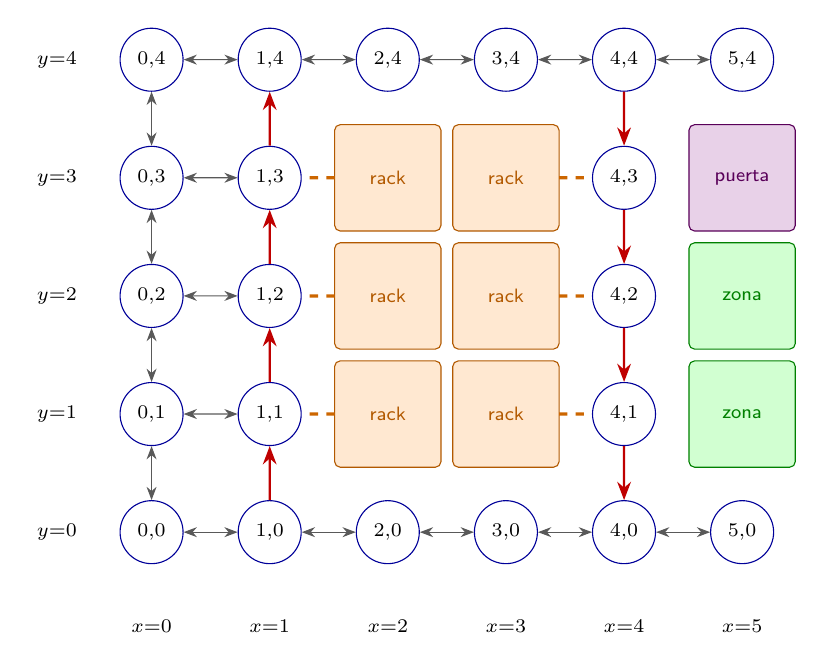
\begin{tikzpicture}[scale=1.5,>=Stealth]
\filldraw[fill=orange!18,draw=orange!70!black,rounded corners=2pt] (1.55,0.55) rectangle (2.45,1.45);
\node[font=\scriptsize\sffamily,text=orange!70!black] at (2,1) {rack};
\filldraw[fill=orange!18,draw=orange!70!black,rounded corners=2pt] (2.55,0.55) rectangle (3.45,1.45);
\node[font=\scriptsize\sffamily,text=orange!70!black] at (3,1) {rack};
\filldraw[fill=orange!18,draw=orange!70!black,rounded corners=2pt] (1.55,1.55) rectangle (2.45,2.45);
\node[font=\scriptsize\sffamily,text=orange!70!black] at (2,2) {rack};
\filldraw[fill=orange!18,draw=orange!70!black,rounded corners=2pt] (2.55,1.55) rectangle (3.45,2.45);
\node[font=\scriptsize\sffamily,text=orange!70!black] at (3,2) {rack};
\filldraw[fill=orange!18,draw=orange!70!black,rounded corners=2pt] (1.55,2.55) rectangle (2.45,3.45);
\node[font=\scriptsize\sffamily,text=orange!70!black] at (2,3) {rack};
\filldraw[fill=orange!18,draw=orange!70!black,rounded corners=2pt] (2.55,2.55) rectangle (3.45,3.45);
\node[font=\scriptsize\sffamily,text=orange!70!black] at (3,3) {rack};
\filldraw[fill=green!18,draw=green!50!black,rounded corners=2pt] (4.55,0.55) rectangle (5.45,1.45);
\node[font=\scriptsize\sffamily,text=green!50!black] at (5,1) {zona};
\filldraw[fill=green!18,draw=green!50!black,rounded corners=2pt] (4.55,1.55) rectangle (5.45,2.45);
\node[font=\scriptsize\sffamily,text=green!50!black] at (5,2) {zona};
\filldraw[fill=violet!18,draw=violet!70!black,rounded corners=2pt] (4.55,2.55) rectangle (5.45,3.45);
\node[font=\scriptsize\sffamily,text=violet!70!black] at (5,3) {puerta};
\node[circle,draw=blue!60!black,fill=white,inner sep=0pt,minimum size=8mm,font=\scriptsize] (n00) at (0,0) {0,0};
\node[circle,draw=blue!60!black,fill=white,inner sep=0pt,minimum size=8mm,font=\scriptsize] (n01) at (0,1) {0,1};
\node[circle,draw=blue!60!black,fill=white,inner sep=0pt,minimum size=8mm,font=\scriptsize] (n02) at (0,2) {0,2};
\node[circle,draw=blue!60!black,fill=white,inner sep=0pt,minimum size=8mm,font=\scriptsize] (n03) at (0,3) {0,3};
\node[circle,draw=blue!60!black,fill=white,inner sep=0pt,minimum size=8mm,font=\scriptsize] (n04) at (0,4) {0,4};
\node[circle,draw=blue!60!black,fill=white,inner sep=0pt,minimum size=8mm,font=\scriptsize] (n10) at (1,0) {1,0};
\node[circle,draw=blue!60!black,fill=white,inner sep=0pt,minimum size=8mm,font=\scriptsize] (n11) at (1,1) {1,1};
\node[circle,draw=blue!60!black,fill=white,inner sep=0pt,minimum size=8mm,font=\scriptsize] (n12) at (1,2) {1,2};
\node[circle,draw=blue!60!black,fill=white,inner sep=0pt,minimum size=8mm,font=\scriptsize] (n13) at (1,3) {1,3};
\node[circle,draw=blue!60!black,fill=white,inner sep=0pt,minimum size=8mm,font=\scriptsize] (n14) at (1,4) {1,4};
\node[circle,draw=blue!60!black,fill=white,inner sep=0pt,minimum size=8mm,font=\scriptsize] (n20) at (2,0) {2,0};
\node[circle,draw=blue!60!black,fill=white,inner sep=0pt,minimum size=8mm,font=\scriptsize] (n24) at (2,4) {2,4};
\node[circle,draw=blue!60!black,fill=white,inner sep=0pt,minimum size=8mm,font=\scriptsize] (n30) at (3,0) {3,0};
\node[circle,draw=blue!60!black,fill=white,inner sep=0pt,minimum size=8mm,font=\scriptsize] (n34) at (3,4) {3,4};
\node[circle,draw=blue!60!black,fill=white,inner sep=0pt,minimum size=8mm,font=\scriptsize] (n40) at (4,0) {4,0};
\node[circle,draw=blue!60!black,fill=white,inner sep=0pt,minimum size=8mm,font=\scriptsize] (n41) at (4,1) {4,1};
\node[circle,draw=blue!60!black,fill=white,inner sep=0pt,minimum size=8mm,font=\scriptsize] (n42) at (4,2) {4,2};
\node[circle,draw=blue!60!black,fill=white,inner sep=0pt,minimum size=8mm,font=\scriptsize] (n43) at (4,3) {4,3};
\node[circle,draw=blue!60!black,fill=white,inner sep=0pt,minimum size=8mm,font=\scriptsize] (n44) at (4,4) {4,4};
\node[circle,draw=blue!60!black,fill=white,inner sep=0pt,minimum size=8mm,font=\scriptsize] (n50) at (5,0) {5,0};
\node[circle,draw=blue!60!black,fill=white,inner sep=0pt,minimum size=8mm,font=\scriptsize] (n54) at (5,4) {5,4};
\draw[<->,gray!70!black] (n00) -- (n01);
\draw[<->,gray!70!black] (n00) -- (n10);
\draw[<->,gray!70!black] (n01) -- (n02);
\draw[<->,gray!70!black] (n01) -- (n11);
\draw[<->,gray!70!black] (n02) -- (n03);
\draw[<->,gray!70!black] (n02) -- (n12);
\draw[<->,gray!70!black] (n03) -- (n04);
\draw[<->,gray!70!black] (n03) -- (n13);
\draw[<->,gray!70!black] (n04) -- (n14);
\draw[->,red!75!black,thick] (n10) -- (n11);
\draw[<->,gray!70!black] (n10) -- (n20);
\draw[->,red!75!black,thick] (n11) -- (n12);
\draw[->,red!75!black,thick] (n12) -- (n13);
\draw[->,red!75!black,thick] (n13) -- (n14);
\draw[<->,gray!70!black] (n14) -- (n24);
\draw[<->,gray!70!black] (n20) -- (n30);
\draw[<->,gray!70!black] (n24) -- (n34);
\draw[<->,gray!70!black] (n30) -- (n40);
\draw[<->,gray!70!black] (n34) -- (n44);
\draw[<->,gray!70!black] (n40) -- (n50);
\draw[->,red!75!black,thick] (n41) -- (n40);
\draw[->,red!75!black,thick] (n42) -- (n41);
\draw[->,red!75!black,thick] (n43) -- (n42);
\draw[->,red!75!black,thick] (n44) -- (n43);
\draw[<->,gray!70!black] (n44) -- (n54);
\draw[orange!80!black,very thick,dashed] (1.55,1) -- (n11);
\draw[orange!80!black,very thick,dashed] (1.55,2) -- (n12);
\draw[orange!80!black,very thick,dashed] (1.55,3) -- (n13);
\draw[orange!80!black,very thick,dashed] (3.45,1) -- (n41);
\draw[orange!80!black,very thick,dashed] (3.45,2) -- (n42);
\draw[orange!80!black,very thick,dashed] (3.45,3) -- (n43);
\node[font=\scriptsize] at (0,-0.8) {$x{=}0$};
\node[font=\scriptsize] at (1,-0.8) {$x{=}1$};
\node[font=\scriptsize] at (2,-0.8) {$x{=}2$};
\node[font=\scriptsize] at (3,-0.8) {$x{=}3$};
\node[font=\scriptsize] at (4,-0.8) {$x{=}4$};
\node[font=\scriptsize] at (5,-0.8) {$x{=}5$};
\node[font=\scriptsize,anchor=east] at (-0.55,0) {$y{=}0$};
\node[font=\scriptsize,anchor=east] at (-0.55,1) {$y{=}1$};
\node[font=\scriptsize,anchor=east] at (-0.55,2) {$y{=}2$};
\node[font=\scriptsize,anchor=east] at (-0.55,3) {$y{=}3$};
\node[font=\scriptsize,anchor=east] at (-0.55,4) {$y{=}4$};
\end{tikzpicture}
\caption{Dígrafo del ejemplo. Gris: pares con ida y vuelta. Rojo: aristas de un solo sentido (la columna $x=1$ sube y la $x=4$ baja). Naranja punteado: celda de rack $\to$ su acceso; la columna izquierda del rack se accede desde $x=1$ y la derecha desde $x=4$.}
\label{fig:ejemplo}
\end{figure}

En la tabla de nodos, la inserción número 13, que corresponde a $(3,0)$, supera $0{,}75\cdot17=12{,}75$ y dispara un rehash a $m=37$. Al final, $\alpha=21/37=0{,}57$ y hay exactamente dos colisiones: la casilla 9 contiene la cadena $(1,2)\to(0,1)$ y la casilla 17, la cadena $(5,0)\to(0,2)$. En cada cadena, el último insertado queda al frente.

%======================================================================
\section{Validación por Componentes Fuertemente Conexas}\label{sec:validacion}

Con manos únicas pueden aparecer \emph{trampas} (zonas a las que se entra y de las que no se sale) o \emph{islas} (zonas a las que no se llega). Ambas situaciones se detectan con las componentes fuertemente conexas (CFC) de $G$.

\begin{algorithm}[H]
\caption{\textsc{Kosaraju-Iterativo}$(G)$}\label{alg:kosaraju}
\begin{algorithmic}[1]
\State $visitado\gets\emptyset$; \ $fin\gets[\,]$
\ForAll{$s\in V$ en orden de inserción, $s\notin visitado$} \Comment{1er DFS sobre $G$}
  \State $visitado\gets visitado\cup\{s\}$; \ $pila\gets[(s,0)]$
  \While{$pila\neq\emptyset$}
    \State $(u,i)\gets$ tope de $pila$
    \If{$i<|ady[u]|$}
      \State reemplazar el tope por $(u,i+1)$; \ $v\gets ady[u][i]$
      \If{$v\notin visitado$} $visitado\gets visitado\cup\{v\}$; \ apilar $(v,0)$ \EndIf
    \Else \ desapilar; \ agregar $u$ al final de $fin$ \Comment{$u$ terminó}
    \EndIf
  \EndWhile
\EndFor
\State $G^T\gets$ tabla hash con $G^T[v]=[\,u : (u,v)\in E\,]$ \Comment{grafo transpuesto}
\State $asignado\gets\emptyset$; \ $comps\gets[\,]$
\ForAll{$r$ en $fin$ recorrido de atrás hacia adelante, $r\notin asignado$} \Comment{2do DFS sobre $G^T$}
  \State $C\gets[\,]$; \ $asignado\gets asignado\cup\{r\}$; \ $pila\gets[r]$
  \While{$pila\neq\emptyset$}
    \State $u\gets$ desapilar; agregar $u$ a $C$
    \ForAll{$v\in G^T[u]$, $v\notin asignado$} $asignado\gets asignado\cup\{v\}$; apilar $v$ \EndFor
  \EndWhile
  \State agregar $C$ a $comps$
\EndFor
\State \Return $comps$ ordenadas de mayor a menor tamaño
\end{algorithmic}
\end{algorithm}

El primer DFS guarda en la pila el índice del próximo sucesor a explorar. Así simula la recursión sin usar la pila de llamadas de Python, cuyo límite (unas mil llamadas) se superaría en almacenes de $200\times200$ con caminos de decenas de miles de celdas.

\paragraph{\textsc{Validar}.} La componente de mayor tamaño se toma como \emph{red principal} $C^\ast$. Luego:
\begin{enumerate}[leftmargin=*]
\item para cada celda de rack con algún acceso en $C^\ast$, ese acceso pasa a ser su acceso principal;
\item si hay más de una CFC, se informa cuántas hay, cuántas celdas quedan fuera de $C^\ast$ y en qué rango de coordenadas;
\item se advierte por cada producto sin acceso o sin acceso en $C^\ast$, por cada zona en la misma situación, y por cada picker cuya posición inicial no es nodo o no está en $C^\ast$.
\end{enumerate}

\paragraph{Ejemplo de trampa.} Si en el ejemplo de la Sección~\ref{sec:ejemplo} el pasillo izquierdo se declara \sS{} y ocupa las columnas 0 y 1, ninguna columna permite subir. Kosaraju devuelve 8 componentes: las dos filas horizontales (6 celdas cada una), los tres pares $\{(0,y),(1,y)\}$ y las tres celdas sueltas de la columna $x=4$. La validación informa que 15 celdas quedan fuera de la red principal, que ambos productos y la zona no tienen acceso en ella y que el picker arranca fuera de ella. Durante el desarrollo, este control detectó una trampa real de 41 celdas en \texttt{escenario{\char95}grande.json}, que se corrigió.

\begin{figure}[H]
\centering
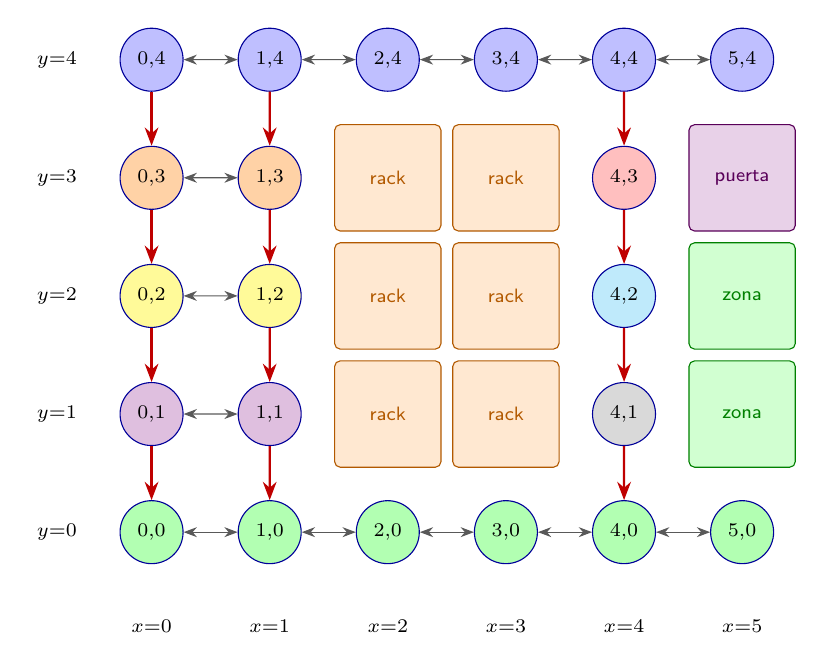
\begin{tikzpicture}[scale=1.5,>=Stealth]
\filldraw[fill=orange!18,draw=orange!70!black,rounded corners=2pt] (1.55,0.55) rectangle (2.45,1.45);
\node[font=\scriptsize\sffamily,text=orange!70!black] at (2,1) {rack};
\filldraw[fill=orange!18,draw=orange!70!black,rounded corners=2pt] (2.55,0.55) rectangle (3.45,1.45);
\node[font=\scriptsize\sffamily,text=orange!70!black] at (3,1) {rack};
\filldraw[fill=orange!18,draw=orange!70!black,rounded corners=2pt] (1.55,1.55) rectangle (2.45,2.45);
\node[font=\scriptsize\sffamily,text=orange!70!black] at (2,2) {rack};
\filldraw[fill=orange!18,draw=orange!70!black,rounded corners=2pt] (2.55,1.55) rectangle (3.45,2.45);
\node[font=\scriptsize\sffamily,text=orange!70!black] at (3,2) {rack};
\filldraw[fill=orange!18,draw=orange!70!black,rounded corners=2pt] (1.55,2.55) rectangle (2.45,3.45);
\node[font=\scriptsize\sffamily,text=orange!70!black] at (2,3) {rack};
\filldraw[fill=orange!18,draw=orange!70!black,rounded corners=2pt] (2.55,2.55) rectangle (3.45,3.45);
\node[font=\scriptsize\sffamily,text=orange!70!black] at (3,3) {rack};
\filldraw[fill=green!18,draw=green!50!black,rounded corners=2pt] (4.55,0.55) rectangle (5.45,1.45);
\node[font=\scriptsize\sffamily,text=green!50!black] at (5,1) {zona};
\filldraw[fill=green!18,draw=green!50!black,rounded corners=2pt] (4.55,1.55) rectangle (5.45,2.45);
\node[font=\scriptsize\sffamily,text=green!50!black] at (5,2) {zona};
\filldraw[fill=violet!18,draw=violet!70!black,rounded corners=2pt] (4.55,2.55) rectangle (5.45,3.45);
\node[font=\scriptsize\sffamily,text=violet!70!black] at (5,3) {puerta};
\node[circle,draw=blue!60!black,fill=green!30,inner sep=0pt,minimum size=8mm,font=\scriptsize] (n00) at (0,0) {0,0};
\node[circle,draw=blue!60!black,fill=violet!25,inner sep=0pt,minimum size=8mm,font=\scriptsize] (n01) at (0,1) {0,1};
\node[circle,draw=blue!60!black,fill=yellow!40,inner sep=0pt,minimum size=8mm,font=\scriptsize] (n02) at (0,2) {0,2};
\node[circle,draw=blue!60!black,fill=orange!35,inner sep=0pt,minimum size=8mm,font=\scriptsize] (n03) at (0,3) {0,3};
\node[circle,draw=blue!60!black,fill=blue!25,inner sep=0pt,minimum size=8mm,font=\scriptsize] (n04) at (0,4) {0,4};
\node[circle,draw=blue!60!black,fill=green!30,inner sep=0pt,minimum size=8mm,font=\scriptsize] (n10) at (1,0) {1,0};
\node[circle,draw=blue!60!black,fill=violet!25,inner sep=0pt,minimum size=8mm,font=\scriptsize] (n11) at (1,1) {1,1};
\node[circle,draw=blue!60!black,fill=yellow!40,inner sep=0pt,minimum size=8mm,font=\scriptsize] (n12) at (1,2) {1,2};
\node[circle,draw=blue!60!black,fill=orange!35,inner sep=0pt,minimum size=8mm,font=\scriptsize] (n13) at (1,3) {1,3};
\node[circle,draw=blue!60!black,fill=blue!25,inner sep=0pt,minimum size=8mm,font=\scriptsize] (n14) at (1,4) {1,4};
\node[circle,draw=blue!60!black,fill=green!30,inner sep=0pt,minimum size=8mm,font=\scriptsize] (n20) at (2,0) {2,0};
\node[circle,draw=blue!60!black,fill=blue!25,inner sep=0pt,minimum size=8mm,font=\scriptsize] (n24) at (2,4) {2,4};
\node[circle,draw=blue!60!black,fill=green!30,inner sep=0pt,minimum size=8mm,font=\scriptsize] (n30) at (3,0) {3,0};
\node[circle,draw=blue!60!black,fill=blue!25,inner sep=0pt,minimum size=8mm,font=\scriptsize] (n34) at (3,4) {3,4};
\node[circle,draw=blue!60!black,fill=green!30,inner sep=0pt,minimum size=8mm,font=\scriptsize] (n40) at (4,0) {4,0};
\node[circle,draw=blue!60!black,fill=gray!30,inner sep=0pt,minimum size=8mm,font=\scriptsize] (n41) at (4,1) {4,1};
\node[circle,draw=blue!60!black,fill=cyan!25,inner sep=0pt,minimum size=8mm,font=\scriptsize] (n42) at (4,2) {4,2};
\node[circle,draw=blue!60!black,fill=red!25,inner sep=0pt,minimum size=8mm,font=\scriptsize] (n43) at (4,3) {4,3};
\node[circle,draw=blue!60!black,fill=blue!25,inner sep=0pt,minimum size=8mm,font=\scriptsize] (n44) at (4,4) {4,4};
\node[circle,draw=blue!60!black,fill=green!30,inner sep=0pt,minimum size=8mm,font=\scriptsize] (n50) at (5,0) {5,0};
\node[circle,draw=blue!60!black,fill=blue!25,inner sep=0pt,minimum size=8mm,font=\scriptsize] (n54) at (5,4) {5,4};
\draw[<->,gray!70!black] (n00) -- (n10);
\draw[->,red!75!black,thick] (n01) -- (n00);
\draw[<->,gray!70!black] (n01) -- (n11);
\draw[->,red!75!black,thick] (n02) -- (n01);
\draw[<->,gray!70!black] (n02) -- (n12);
\draw[->,red!75!black,thick] (n03) -- (n02);
\draw[<->,gray!70!black] (n03) -- (n13);
\draw[->,red!75!black,thick] (n04) -- (n03);
\draw[<->,gray!70!black] (n04) -- (n14);
\draw[<->,gray!70!black] (n10) -- (n20);
\draw[->,red!75!black,thick] (n11) -- (n10);
\draw[->,red!75!black,thick] (n12) -- (n11);
\draw[->,red!75!black,thick] (n13) -- (n12);
\draw[->,red!75!black,thick] (n14) -- (n13);
\draw[<->,gray!70!black] (n14) -- (n24);
\draw[<->,gray!70!black] (n20) -- (n30);
\draw[<->,gray!70!black] (n24) -- (n34);
\draw[<->,gray!70!black] (n30) -- (n40);
\draw[<->,gray!70!black] (n34) -- (n44);
\draw[<->,gray!70!black] (n40) -- (n50);
\draw[->,red!75!black,thick] (n41) -- (n40);
\draw[->,red!75!black,thick] (n42) -- (n41);
\draw[->,red!75!black,thick] (n43) -- (n42);
\draw[->,red!75!black,thick] (n44) -- (n43);
\draw[<->,gray!70!black] (n44) -- (n54);
\node[font=\scriptsize] at (0,-0.8) {$x{=}0$};
\node[font=\scriptsize] at (1,-0.8) {$x{=}1$};
\node[font=\scriptsize] at (2,-0.8) {$x{=}2$};
\node[font=\scriptsize] at (3,-0.8) {$x{=}3$};
\node[font=\scriptsize] at (4,-0.8) {$x{=}4$};
\node[font=\scriptsize] at (5,-0.8) {$x{=}5$};
\node[font=\scriptsize,anchor=east] at (-0.55,0) {$y{=}0$};
\node[font=\scriptsize,anchor=east] at (-0.55,1) {$y{=}1$};
\node[font=\scriptsize,anchor=east] at (-0.55,2) {$y{=}2$};
\node[font=\scriptsize,anchor=east] at (-0.55,3) {$y{=}3$};
\node[font=\scriptsize,anchor=east] at (-0.55,4) {$y{=}4$};
\end{tikzpicture}
\caption{Escenario con trampa: cada color es una componente fuertemente conexa. Ninguna arista sube, por lo que desde abajo no se puede volver a la fila superior.}
\label{fig:trampa}
\end{figure}

%======================================================================
\section{Taxonomía de Casos de Construcción}

\subsection{Caso 1: Cruce de Pasillos}
\textbf{Condición:} una celda está cubierta por dos o más pasillos.\\
\textbf{Resolución:} los pasillos se procesan en el orden del JSON. Si la celda ya tiene \sA, lo conserva; si no, toma el sentido del pasillo actual. Así, si algún pasillo \sA{} la cubre, el cruce queda \sA{} y se puede doblar; si ninguno es \sA, queda el sentido del último declarado. Cada cruce genera además una advertencia informativa ``pisa''.

\subsection{Caso 2: Piso Libre no Declarado}
\textbf{Condición:} una celda no es obstáculo ni pertenece a ningún pasillo.\\
\textbf{Resolución:} es nodo con $\sigma=\sA$ y sin identificador de pasillo. Un escenario sin pasillos declarados es, por lo tanto, una grilla completamente bidireccional.

\subsection{Caso 3: Obstáculo sobre un Pasillo o sobre Otro Obstáculo}
\textbf{Condición:} un rack, zona o puerta ocupa una celda ya ocupada.\\
\textbf{Resolución:} se emite la advertencia ``pisa''. Como los nodos se crean consultando primero la tabla de obstáculos, la celda queda como obstáculo y no como nodo. (El validador previo ya rechaza obstáculos superpuestos entre sí.)

\subsection{Caso 4: Forma del Rack}
\textbf{Condición:} rack vertical ($a_R=2$), horizontal ($h_R=2$), cuadrado de $2\times2$ o sin ningún lado igual a 2.\\
\textbf{Resolución:} se aplica $\mathcal{D}_R$ de la Sección~\ref{sec:accesos}. El rack cuadrado se accede por cualquier lado. El rack sin lado 2 es rechazado por el validador; si llegara a la construcción, emite una advertencia y se accede por cualquier lado.

\subsection{Caso 5: Trampas e Islas}
\textbf{Condición:} $G$ tiene más de una CFC.\\
\textbf{Resolución:} el almacén se construye igual, se advierte y se priorizan los accesos dentro de la red principal. Los módulos de ruteo trabajan sobre el mismo grafo, por lo que nunca se elige como destino un acceso al que no se podría llegar si existe otro que sí sirve.

\subsection{Caso 6: Producto o Zona sin Acceso}
\textbf{Condición:} todos los vecinos del costado largo de una celda de rack son obstáculos, o ninguno está en $C^\ast$; o una zona no tiene pasillos adyacentes.\\
\textbf{Resolución:} advertencia específica por producto y por zona. El armado de waves puede consultarlo en $O(1)$ con \texttt{accesos{\char95}rack{\char95}a{\char95}pasillo}.

\subsection{Caso 7: Picker sobre un Obstáculo}
\textbf{Condición:} la posición inicial no es un nodo.\\
\textbf{Resolución:} la validación lo advierte con la posición original y luego el picker se reubica en el acceso correspondiente (Paso 10).

\subsection{Caso 8: Datos Fuera de Rango o Mal Formados}
\textbf{Condición:} campos faltantes, tipos incorrectos, elementos fuera del mapa o sentido inexistente.\\
\textbf{Resolución:} \textbf{error} con mensaje claro (del validador o de \textsc{Ocupar}); no se construye un almacén inconsistente.

%======================================================================
\section{Demostraciones y Análisis Asintótico}

\subsection{Demostración 1: Inyectividad de la Codificación de Coordenadas}

\begin{lema}\label{lema:prehash}
Si $0\le y,y'<B$ y $0\le x,x'$ con $xB+y<p$, entonces $k(x,y)=k(x',y')\Rightarrow(x,y)=(x',y')$. En particular, la codificación \eqref{eq:prehash} es inyectiva sobre todas las coordenadas válidas ($x,y\le199$).
\end{lema}
\begin{proof}
Si $xB+y=x'B+y'$, reduciendo módulo $B$ se obtiene $y\equiv y'\pmod B$ y, como $0\le y,y'<B$, resulta $y=y'$. Entonces $xB=x'B$ y $x=x'$. Para coordenadas válidas, $k\le199\cdot1\,000\,003+199<2^{61}-1=p$, por lo que la reducción módulo $p$ no altera el valor y la composición sigue siendo inyectiva.
\end{proof}

Gracias a este lema, dos celdas distintas nunca comparten clave entera. Las únicas colisiones posibles provienen de la reducción módulo $m$ de la Etapa~2, y son las que resuelve el encadenamiento.

\subsection{Demostración 2: Universalidad de la Familia $h_{a,b}$}

\begin{teorema}[Carter y Wegman; CLRS, Teorema 11.5]\label{teo:universal}
Sea $p$ primo y $\mathcal{H}=\{h_{a,b} : a\in\mathbb{Z}_p^\ast,\ b\in\mathbb{Z}_p\}$. Para todo par de claves distintas $k\neq l$ en $\mathbb{Z}_p$,
\[ \Pr_{a,b}\bigl[h_{a,b}(k)=h_{a,b}(l)\bigr]\le\frac{1}{m}. \]
\end{teorema}
\begin{proof}
Sean $r=(ak+b)\bmod p$ y $s=(al+b)\bmod p$. Entonces $r-s\equiv a(k-l)\pmod p$. Como $p$ es primo, $a\not\equiv0$ y $k\not\equiv l$, el producto no es nulo módulo $p$, así que $r\neq s$: \textbf{antes de reducir módulo $m$ no hay colisiones}.

Además, el sistema $r\equiv ak+b$, $s\equiv al+b$ tiene solución única $a=(r-s)(k-l)^{-1}$, $b=r-ak$ en $\mathbb{Z}_p$. Por lo tanto, la función $(a,b)\mapsto(r,s)$ es una biyección entre los $p(p-1)$ pares con $a\neq0$ y los $p(p-1)$ pares $(r,s)$ con $r\neq s$. Elegir $(a,b)$ uniformemente equivale entonces a elegir $(r,s)$ uniformemente entre los pares con $r\ne s$.

Hay colisión si y solo si $r\equiv s\pmod m$. Fijado $r$, la cantidad de valores $s\neq r$ en $\{0,\dots,p-1\}$ con $s\equiv r\pmod m$ es a lo sumo $\lceil p/m\rceil-1\le (p-1)/m$. Entonces la probabilidad de colisión es a lo sumo $\frac{(p-1)/m}{p-1}=\frac1m$.
\end{proof}

Por el Lema~\ref{lema:prehash}, las claves de dos celdas distintas son enteros distintos menores que $p$, de modo que el teorema se aplica directamente. La consecuencia práctica es que no existe un conjunto de coordenadas que sea ``malo'' de antemano para la tabla, cosa que sí ocurre con el método de la división $k\bmod m$ ante claves con patrones regulares.

\textit{Observación.} La garantía es probabilística sobre la elección de $(a,b)$. Al fijar la semilla, la tabla es determinista; la elección de la semilla 318 se verificó empíricamente sobre todos los escenarios (Tabla~\ref{tab:escenarios}).

\subsection{Demostración 3: Costo Esperado Constante con Encadenamiento}

\begin{teorema}\label{teo:esperado}
Con una función elegida de una familia universal y factor de carga $\alpha=n/m$, la longitud esperada de la cadena que recorre una búsqueda es a lo sumo $1+\alpha$. Como la tabla mantiene $\alpha\le0{,}75$, buscar, insertar y borrar cuestan $O(1)$ esperado.
\end{teorema}
\begin{proof}
Sea $k$ la clave buscada y, para cada otra clave $l$ almacenada, sea $X_{l}$ la variable indicadora de $h(l)=h(k)$. La cadena de la casilla de $k$ tiene longitud $L=[k\in T]+\sum_{l\neq k}X_{l}$. Por linealidad de la esperanza y el Teorema~\ref{teo:universal},
\[ \mathbb{E}[L]\le 1+\sum_{l\neq k}\Pr[h(l)=h(k)]\le 1+\frac{n}{m}=1+\alpha. \]
Calcular $h$ cuesta $O(1)$ para coordenadas, y la búsqueda recorre a lo sumo esa cadena. Insertar es una búsqueda más un enlace al frente, y borrar es una búsqueda más un desenlace.
\end{proof}

\begin{teorema}\label{teo:amortizado}
Una sucesión de $n$ inserciones, con rehash al primo siguiente a $2m$ cada vez que $n>0{,}75m$, cuesta $O(n)$ en total. Es decir, cada inserción cuesta $O(1)$ amortizado.
\end{teorema}
\begin{proof}
Cada rehash al pasar de $m_i$ a $m_{i+1}\ge2m_i$ reinserta $n_i\le0{,}75\,m_i+1$ claves y crea $m_{i+1}$ casillas: cuesta $O(m_{i+1})$. Como los tamaños al menos se duplican, $\sum_i m_{i+1}\le 2\,m_{\text{final}}$. Además $m_{\text{final}}=O(n)$: por el postulado de Bertrand el primo siguiente a $2m$ es menor que $4m$, y el último rehash ocurrió con $m<\tfrac{4}{3}n$. El costo total de los rehash es entonces $O(n)$, y sumado al $O(1)$ esperado de cada inserción da $O(n)$.
\end{proof}

\subsection{Demostración 4: Correctitud del Dígrafo Construido}

\begin{teorema}\label{teo:digrafo}
Al terminar \textsc{Construir-Dígrafo}, el conjunto de claves de \texttt{nodos} es exactamente $V$, y $v\in ady[u]$ si y solo si $(u,v)\in E$.
\end{teorema}
\begin{proof}
\emph{Nodos.} El primer doble ciclo recorre cada $c\in\Omega$ exactamente una vez y la inserta si y solo si $c\notin\mathcal{O}$, es decir, si $c\in V$.

\emph{Aristas, $(\Leftarrow)$.} Sea $(u,v)\in E$, con $v=u+\delta$. Al procesar $u$, el ciclo interno recorre todo $\delta\in D(\sigma(u))$; en ese momento $v\in nodos$ (todos los nodos se crearon antes) y $\neg\CM(\delta,\sigma(v))$, así que $v$ se agrega si no estaba.

\emph{Aristas, $(\Rightarrow)$.} El único punto donde se agrega $v$ a $ady[u]$ exige $\delta\in D(\sigma(u))$, $v\in nodos=V$ y $\neg\CM(\delta,\sigma(v))$, que son exactamente las condiciones de la definición de $E$.

Como se controla $v\notin ady[u]$ antes de agregar, no hay aristas repetidas, y por lo tanto $|ady[u]|\le|D(\sigma(u))|\le4$.
\end{proof}

\subsection{Demostración 5: Correctitud y Costo de Kosaraju}

\begin{teorema}[CLRS, Teorema 22.16]
El Algoritmo~\ref{alg:kosaraju} devuelve exactamente las componentes fuertemente conexas de $G$, en tiempo $\Theta(|V|+|E|)=\Theta(|V|)$ esperado, más $O(c\log c)$ para ordenar las $c$ componentes por tamaño.
\end{teorema}
\begin{proof}[Esquema]
\emph{Correctitud.} El DFS iterativo visita y finaliza los nodos en el mismo orden que el recursivo, porque el par $(u,i)$ reproduce exactamente el estado de cada llamada. Por el lema de tiempos de finalización (CLRS, Lema 22.14), si $C\neq C'$ son CFC y existe una arista de $C$ a $C'$, entonces $f(C)>f(C')$, donde $f$ es el máximo tiempo de finalización de la componente. Luego, el nodo de mayor finalización pertenece a una componente $C_1$ sin aristas entrantes desde otras componentes aún no asignadas. En $G^T$, las aristas de $C_1$ hacia afuera quedan invertidas, así que el DFS iniciado en ese nodo alcanza exactamente $C_1$ (las CFC de $G$ y de $G^T$ coinciden). Por inducción sobre las componentes ya asignadas, cada árbol del segundo DFS es una CFC.

\emph{Costo.} Cada nodo se apila una vez en cada DFS y cada arista se examina una vez en cada DFS y una vez al construir $G^T$. Cada consulta a las tablas hash es $O(1)$ esperado (Teorema~\ref{teo:esperado}). El total es $\Theta(|V|+|E|)$ y, como $|E|\le4|V|$, $\Theta(|V|)$. El ordenamiento final agrega $O(c\log c)$, que es $O(1)$ en los escenarios válidos ($c=1$).
\end{proof}

\begin{lema}[Garantía para los módulos de ruteo]
Si $G$ tiene una sola CFC, para todo par de nodos $u,v$ existe un camino dirigido de $u$ a $v$ y otro de $v$ a $u$. En consecuencia, todo producto con acceso, toda zona con acceso y todo picker ubicado en un nodo son mutuamente alcanzables, y Dijkstra encuentra siempre una ruta finita.
\end{lema}
\begin{proof}
Es la definición de componente fuertemente conexa aplicada a $C^\ast=V$. Los accesos y las posiciones de los pickers son nodos de $V$.
\end{proof}

\subsection{Demostración 6: Linealidad de la Construcción Completa}

\begin{teorema}
Sean $W\cdot H$ el área, $A$ la suma de las áreas de los rectángulos declarados, $P$ la cantidad de productos, $n$ la de pedidos con $L$ ítems como máximo y $K$ la de pickers. \textsc{Construir-Almacén} cuesta $\Theta(W\cdot H+A+P+nL+K)$ en tiempo esperado. Como los obstáculos no se superponen y los pasillos solo se superponen en los cruces, $A=O(W\cdot H)$ y el costo es lineal en el área.
\end{teorema}
\begin{proof}
Marcar pasillos y obstáculos visita $A$ celdas en total. Cada celda visitada realiza $O(1)$ operaciones esperadas sobre tablas hash. Los productos cuestan $\Theta(P)$. El ciclo de nodos es $\Theta(W\cdot H)$. El de accesos y aristas es $O(|V|\cdot|\Delta|)=O(W\cdot H)$. Kosaraju es $\Theta(|V|)$. La validación recorre accesos ($O(W\cdot H)$), productos, zonas y pickers. Los pedidos cuestan $\Theta(nL)$ y los pickers $\Theta(K)$. El espacio está dominado por las tablas, de tamaño $\Theta(|V|+|E|+|\mathcal{O}|)=\Theta(W\cdot H)$, más los datos de negocio.
\end{proof}

%======================================================================
\section{Resultados Experimentales}

Las mediciones se tomaron con el código del proyecto (mediana de 5 corridas; Python~3, sin librerías externas).

\begin{table}[H]
\centering\small
\begin{tabular}{@{}lrrrrrrrr@{}}
\toprule
Escenario & $W\times H$ & $|V|$ & $|E|$ & CFC & $m$ & $\alpha$ & cad.\ máx. & construir \\
\midrule
\texttt{escenario{\char95}basico} & $18\times16$ & 230 & 692 & 1 & 331 & 0{,}69 & 2 & 6{,}2 ms\\
\texttt{gen{\char95}chico} & $10\times29$ & 207 & 514 & 1 & 331 & 0{,}63 & 2 & 5{,}7 ms\\
\texttt{gen{\char95}mediano} & $26\times37$ & 652 & 1678 & 1 & 1361 & 0{,}48 & 2 & 18{,}3 ms\\
\texttt{escenario{\char95}grande} & $60\times40$ & 1898 & 6048 & 1 & 2729 & 0{,}70 & 2 & 56{,}0 ms\\
\texttt{gen{\char95}grande} & $42\times85$ & 2396 & 6226 & 1 & 5471 & 0{,}44 & 2 & 86{,}2 ms\\
\bottomrule
\end{tabular}
\caption{Escenarios del proyecto: tamaño del dígrafo, estado de la tabla de nodos y tiempo de construcción completa. Ninguna cadena supera los 2 elementos y todos los escenarios forman una única CFC.}
\label{tab:escenarios}
\end{table}

Para medir la escalabilidad se generaron almacenes de $n\times n$ con racks verticales separados por pasillos de mano única alternada y dos franjas horizontales \sA. Se comparó además la tabla propia contra el diccionario nativo de Python (reemplazándolo solo para la medición), verificando que ambos producen el mismo grafo.

\begin{table}[H]
\centering\small
\begin{tabular}{@{}rrrrrrrr@{}}
\toprule
$n$ & celdas & $|V|$ & construir (propia) & $\mu$s/celda & Kosaraju (propia) & construir (\texttt{dict}) & factor\\
\midrule
25 & 625 & 331 & 9{,}5 ms & 15{,}2 & 2{,}1 ms & 2{,}5 ms & $\times3{,}9$\\
50 & 2\,500 & 1\,028 & 30{,}8 ms & 12{,}3 & 6{,}2 ms & 7{,}6 ms & $\times4{,}1$\\
100 & 10\,000 & 3\,856 & 127{,}4 ms & 12{,}7 & 21{,}3 ms & 37{,}0 ms & $\times3{,}4$\\
150 & 22\,500 & 8\,192 & 400{,}7 ms & 17{,}8 & 46{,}8 ms & 104{,}5 ms & $\times3{,}8$\\
200 & 40\,000 & 14\,128 & 787{,}3 ms & 19{,}7 & 88{,}0 ms & 210{,}3 ms & $\times3{,}7$\\
\bottomrule
\end{tabular}
\caption{Escalabilidad. Al multiplicar el área por 64, el tiempo se multiplica por 83, y el costo por celda se mantiene en el mismo orden (12--20\,$\mu$s), lo que es consistente con $\Theta(W\cdot H)$. Kosaraju crece igual que $|V|$.}
\label{tab:escala}
\end{table}

La tabla propia es entre 3,4 y 4,1 veces más lenta que \texttt{dict}, y ese factor se mantiene \textbf{constante} con el tamaño. Esto es lo esperado: ambas son $O(1)$ esperado por operación, pero \texttt{dict} está implementado en C y la tabla propia en Python. El costo absoluto (menos de un segundo para el máximo permitido de $200\times200$) se paga una sola vez al cargar el escenario. Las consultas posteriores son $O(1)$ esperado. La implementación se verifica con 6 pruebas específicas dentro de la suite del proyecto (60 pruebas, todas exitosas): equivalencia con un diccionario en 4\,000 operaciones aleatorias incluyendo el orden de iteración, fórmula y determinismo de $h_{a,b}$, inyectividad de las coordenadas, encadenamiento ante colisiones forzadas, invariante $\alpha\le0{,}75$ con $m$ primo, y que el dígrafo construido coincide con el esperado.

%======================================================================
\section{Cuadro Resumen de Complejidades Computacionales}

Notación: $W\cdot H$ área del almacén, $A=O(W\cdot H)$ suma de áreas declaradas, $V$ nodos de pasillo, $E\le4V$ aristas, $P$ productos, $n$ pedidos con hasta $L$ ítems, $K$ pickers, $n_T$ claves de una tabla hash.

\begin{table}[H]
\centering\small
\begin{tabularx}{\textwidth}{@{}>{\raggedright\arraybackslash}p{3.6cm}>{\centering\arraybackslash}p{3.2cm}>{\centering\arraybackslash}p{1.7cm}>{\raggedright\arraybackslash}X@{}}
\toprule
\textbf{Operación / Algoritmo} & \textbf{Tiempo} & \textbf{Espacio} & \textbf{Justificación}\\
\midrule
Codificar coordenada y $h_{a,b}$ & $\Theta(1)$ & $O(1)$ & Aritmética entera; inyectiva (Lema~\ref{lema:prehash}).\\
Buscar / insertar / borrar en tabla & $O(1)$ esp., $O(n_T)$ peor & $\Theta(n_T+m)$ & Hashing universal + encadenamiento, $\alpha\le0{,}75$ (Teorema~\ref{teo:esperado}).\\
Rehash & $\Theta(n_T+m)$; $O(1)$ amort. & $\Theta(m)$ & Duplicación a tamaño primo (Teorema~\ref{teo:amortizado}).\\
Recorrer la tabla & $\Theta(n_T)$ & $O(1)$ & Arreglo de entradas en orden de inserción.\\
Marcar pasillos y obstáculos & $\Theta(W\cdot H)$ esp. & $\Theta(W\cdot H)$ & Una operación de tabla por celda de cada rectángulo.\\
Crear nodos & $\Theta(W\cdot H)$ esp. & $\Theta(V)$ & Barrido completo de la grilla.\\
Accesos y aristas & $\Theta(V)$ esp. & $\Theta(V+E)$ & Cuatro vecinos por nodo, $E\le4V$ (Teorema~\ref{teo:digrafo}).\\
Kosaraju iterativo & $\Theta(V+E)=\Theta(V)$ & $\Theta(V)$ & Dos DFS con pila propia + transpuesto (+$O(c\log c)$ al ordenar $c$ CFC).\\
Validación & $O(V+P+K)$ & $O(V)$ & Pertenencia a $C^\ast$ en $O(1)$ con conjunto.\\
Construcción completa & $\Theta(W\cdot H+A+P+nL+K)$ & ídem & Suma de las etapas; lineal en la entrada.\\
Sucesores de un nodo & $O(1)$ esp. & --- & Una consulta a \texttt{lista{\char95}adyacencia}.\\
Acceso de un producto & $O(1)$ esp. & --- & Catálogo + \texttt{acceso{\char95}rack{\char95}a{\char95}pasillo}.\\
\bottomrule
\end{tabularx}
\caption{Resumen asintótico de la capa de modelado.}
\end{table}

%======================================================================
\section{Conclusión}

El almacén se modela como un dígrafo ralo de celdas de pasillo, construido en tiempo lineal en el área, cuya regla de aristas codifica con precisión la circulación de mano única y los giros en los cruces. Los accesos a racks y zonas se precalculan respetando que los racks se operan por su costado largo, de modo que el resto del sistema resuelve en tiempo constante dónde detener a un picker. Toda la topología reside en una tabla hash propia con hashing universal, encadenamiento y redimensionamiento a tamaño primo. Esto cumple con la exigencia de implementar las estructuras principales, con garantías demostradas de costo esperado constante, orden de iteración determinista y cadenas de longitud máxima 2 en todos los escenarios. Finalmente, Kosaraju certifica que el mapa forma una única componente fuertemente conexa, lo que garantiza que el armado de waves y el ruteo con Dijkstra siempre trabajan sobre ubicaciones mutuamente alcanzables, y detecta trampas e islas antes de simular.

\end{document}
